\documentclass[text.tex]{subfiles}

\begin{document}

\section{Quasicrystal}\label{sec_quasicrystalEaseIn}%---------------------------------------------------
Unfortunately, there is so far no established mathematical definition of a quasicrystal, in the most basic terms it is just a set that is ordered but not periodic. 

We are going to introduce our own attributes that a set $\Lambda\subset\CC$ needs to have to be a quasicrystal. 

First we require $\Lambda$ to be not too dense but also not too discrete. In other words to have uniform discreetness as well as finite density. 

\begin{enumerate}
\item uniform discreteness: $$\exists\,r_1>0,\; \forall z_1,z_2\in\Lambda, z_1\neq z_2:\; |z_1-z_2|>r_1$$
\item relative density: $$\exists\,r_2>0,\; \forall z\in\CC:\; B(z,r_2)\cap\Lambda \neq \emptyset$$
\end{enumerate}

Next we want finite local complexity. Sometimes this attribute is written as finiteness of the set of intersections of $\Lambda$ with balls of fixed but arbitrary radius centered at any point of $\Lambda$:
$$\forall\,\rho>0:\;\big|\{\Lambda\cap B(x,\rho)\;|\;\forall x\in\Lambda\}\big| < \infty$$
However since we are going to study the Voronoi diagram of $\Lambda$ we directly require the list of Voronoi tiles of $\Lambda$ to be finite. 

\begin{enumerate}
\setcounter{enumi}{2}
\item finite local complexity: $$\big|\{V(x)-x\,|\, x\in \Lambda\}\big|<\infty$$
\end{enumerate}

So far we have achieved the orderedness part but even periodic lattices have these properties. To break the periodicity we are going to require non-crystallographic rotational symmetry and nontrivial dilation.  

\begin{enumerate}
\setcounter{enumi}{3}
\item rotational symmetry: $$\exists\,\zeta = e^{2\pi \i/n},\,n\in\NN\setminus\{2,3,4,6\}:\; \zeta\Lambda = \Lambda$$
\item dilation: $$\exists\,\beta\in\RR\setminus\{-1,1\}:\; \beta\Lambda\subset \Lambda$$
\end{enumerate}

It stems form these properties alone, that among other constants a quasicrystal is linked to a root of unity $\zeta$ and to a number $\beta\in\RR\setminus\{-1,1\}$. Of course not every pair $(\zeta, \beta)$ is associated with a quasicrystal.

In the next section we will go through parameters $\zeta$ and $\beta$ which are associated with a quasicrystal and we will explain where do they come from. 

\section{Pisot-cyclotomic numbers}\label{sec_pisotCyclotomic}%--------------------------------------------------------
Pisot-cyclotomic numbers are Pisot numbers and are algebraically related to roots of unity. We will use these numbers in place of $\beta$ from previous section. 

\begin{definition}\label{def_pisotCyclotomic}
Let $\rho = 2\cos\left(2\pi/n\right)$ for a given $n>4$, its extension ring $\ring[\rho]$ and $m$ order of $\rho$. A \textbf{Pisot-cyclotomic} number of degree $m$, of order $n$ associated to $\rho$ is a Pisot number $\beta \in \ring[\rho]$ such that
$$\ring = \ring[\rho]$$
\end{definition}

Nontrivial $n$th root of unity $\zeta = e^{2\pi \i/n}$ is by definition a solution to equation
$$\frac{\zeta^n-1}{\zeta-1} = \zeta^{n-1}+\zeta^{n-2}+\dots+\zeta+1 = 0$$
further for $\rho = 2\cos\left(2\pi/n\right)$ it holds
$$\rho = \zeta + \bar{\zeta}\quad\Rightarrow\quad \zeta^2 = \rho\zeta - 1$$
Therefore for extension rings $\ring[\zeta]$ and $\ring[\rho]$ we have
$$\ring[\zeta] = \ring[\rho] + \ring[\rho]\zeta$$
and finally for Pisot-cyclotomic $\beta$ associated to $\rho$ we acquire
$$\ring[\zeta] = \ring + \ring\zeta$$
Such countable ring is of course $n$-fold rotationally invariant
$$\zeta^k\ring[\zeta] \subset \ring[\zeta]\qquad k\in\widehat{n-1}$$

To summarize $\beta$ is Pisot (and thus real) and it can be used to decompose $n$-fold rotationally invariant complex ring $\ring[\zeta]$ as $\ring + \ring\zeta$. 

For further work we will need actual values of Pisot-cyclotomic numbers and so in the next section we will show a method for finding quadratic Pisot-cyclotomic numbers, whose quasicrystals we will later analyze. The method could of course be generalized to different degrees. 

\subsection{Quadratic Pisot-cyclotomic numbers}
\begin{remark}
Even though we are mainly focusing on two dimensional quasicrystals, that is not dictated by the quadratic-ness of $\beta$. Quadratic Pisot-cyclotomic numbers are also associated to quasicrystals of arbitrary dimension. 
\end{remark}

As stated in preliminaries, the degree of root of unity of order $n$ is $\varphi(n)$ (where $\varphi$ is the Euler function). From the decomposition in the previous section we can easily infer that the degree of $\zeta$ is double of degree of $\beta$ (or $\rho$). Moreover, we are looking for $\beta$ of degree $2$. Together we acquire the following equation. 
$$\varphi(n) = 2\cdot 2 = 4$$
With help from the Euler product formula we can show that such equation holds only for $n\in\{5,8,10,12\}$. 

For each $n\in\{5,8,10,12\}$ there is $\rho = 2\cos\left(2\pi/n\right)$ and for each such $\rho$ there are $\beta \in \ring[\rho]$ following Definition \ref{def_pisotCyclotomic}. Each of these numbers $\beta$ is associated to the same quasicrystal and so it is sufficient to pick only one representative. 

Moreover, since $2\cos\left(2\pi/5\right) = \frac{\sqrt{5}-1}{2} = \frac{\sqrt{5}+1}{2} -1 = 2\cos\left(2\pi/10\right) - 1$ the extension rings $\ring[2\cos\left(2\pi/5\right)]$ and $\ring[2\cos\left(2\pi/10\right)]$ are identical and by extension the quasicrystals associated are also the same. Therefore we can skip the $5$-fold rotational symmetry. 

To summarize, quadratic Pisot-cyclotomic numbers $\beta$ can only be associated to quasicrystals with $8$-fold, $10$-fold or $12$-fold rotational symmetries. Table \ref{tab_quadraticPisotCyclotomic} shows a list of quadratic Pisot-cyclotomic numbers interesting for Quasicrystallography. 

\begin{table}[h!]
\centering
\begin{tabular}{cccc}
$n$ & $\rho$ & $\beta$ & $\zeta$ \\
\hline
$8$  & $2 \cos\left(\frac{2\pi}{8}\right)$  & $ 1+\sqrt{2} $          & $e^{2i\pi/8}$  \\
$10$ & $2 \cos\left(\frac{2\pi}{10}\right)$ & $\frac{1+\sqrt{5}}{2} $ & $e^{2i\pi/10}$ \\
$12$ & $2 \cos\left(\frac{2\pi}{12}\right)$ & $ 2+\sqrt{3} $          & $e^{2i\pi/12}$ \\
\end{tabular}
\caption{Pisot-cyclotomic numbers of degree $2$, of order $n$, associated to $\rho$.}
\label{tab_quadraticPisotCyclotomic}
\end{table}

Now we want to explore the connection between Galois isomorphisms of $\zeta$ and $\beta$. As we have shown here and in Section \ref{sec_rootOfUnity}, for quadratic Pisot-cyclotomic $\beta$ the associated root of unity $\zeta$ is of degree $4$ and among its four Galois isomorphisms there are two that do not change the real part of $\zeta$. Consequently they also do not alter $\rho = \zeta +\bar{\zeta} = 2\Re{(\zeta)}$ and by extension neither they alter $\rho$'s extension ring $\ring[\rho]$. By further extension these two Galois isomorphisms of $\zeta$ also do not change $\beta\in\ring=\ring[\rho]$. 

It turns out that the other two Galois isomorphisms of $\zeta$ do change $\beta$ to its conjugate root $\beta'$, these two are important for our model of the quasicrystal, which we will present in the next section. 

\section{Quasicrystal model}%--------------------------------------------------------------------------------
There certainly are many ways to acquire a set that follows the attributes listed in Section \ref{sec_quasicrystalEaseIn}. We utilize the cut-and-project scheme described in Section \ref{sec_cutAndProject}. 

Even though we showed the two dimensional quasicrystal as a subset of $\CC$ it is sometimes preferable to treat it as a subset of $\RR^2$. Thus we present two definitions of our model of a quasicrystal, one in $\CC$ (Definition \ref{def_quasicrystalComplex}) and one in $\RR^2$ (Definition \ref{def_quasicrystal}). 

\begin{definition}\label{def_quasicrystalComplex}
Let $n\in\NN\setminus\{2,3,4,6\}$. Let $\beta$ be a quadratic Pisot-cyclotomic number of order $n$, associated to $\rho = 2\cos\left(2\pi/n\right)$ (and $\zeta = e^{2\pi \i/n}$). 
Further, let $\ast^\CC$ be a Galois isomorphism of $\zeta$, such that $\beta^{\ast^\CC} = \beta'$. 
Let  $M^\CC = \ring+\ring\zeta$ and $N^\CC=\ring[\zeta^{\ast^\CC}]$.
Lastly, let $\Omega^\CC\subset N^\CC$ be bounded with nonempty interior. 
The \textbf{complex model of two dimensional quasicrystal linked to irrationality $\beta$ and window $\Omega^\CC$} is the set:
$$\quasi{\Omega^\CC} = \{ x \in M^\CC\; |\; x^{\ast^\CC}\in \Omega^\CC\}$$
\end{definition}

Following Definition \ref{def_quasicrystal} uses objects defined in Definition \ref{def_quasicrystalComplex}. 

\begin{definition}\label{def_quasicrystal}
Let $n\in\NN\setminus\{2,3,4,6\}$. Let $\beta$ be a quadratic Pisot-cyclotomic number of order $n$, associated to $\rho = 2\cos\left(2\pi/n\right)$ (and $\zeta = e^{2\pi \i/n}$). 
Further, let $\ast:\RR^2\to\RR^2$ be defined as $(x,y)^\ast = (\Re{\big((x+iy)^{\ast^\CC}\big)}, \Im{\big((x+iy)^{\ast^\CC}\big)})$. 
Let $v_1, v_2\in\RR^2$:
$$v_1=(1,0)\quad\text{and}\quad v_2 = (\Re{(\zeta)}, \Im{(\zeta)})$$
Let $M = \ring v_1+\ring v_2$ and similarly let $N = \ring v_1^\ast+\ring v_2^\ast$.
Lastly, let $\Omega\subset N$ be bounded with nonempty interior. 
The \textbf{model of two dimensional quasicrystal linked to irrationality $\beta$ and window $\Omega$} is the set:
$$\quasi{\Omega} = \{ x \in M\; |\; x^\ast\in \Omega\}$$
\end{definition}

So far the entire theses was purely abstract. To illustrate what a quasicrystal might look like, there is Figure \ref{fig_quasicrystalFirstExample} which shows finite section of a two dimensional quasicrystal with $8$-fold rotational symmetry.

\begin{figure}[h]
\centering
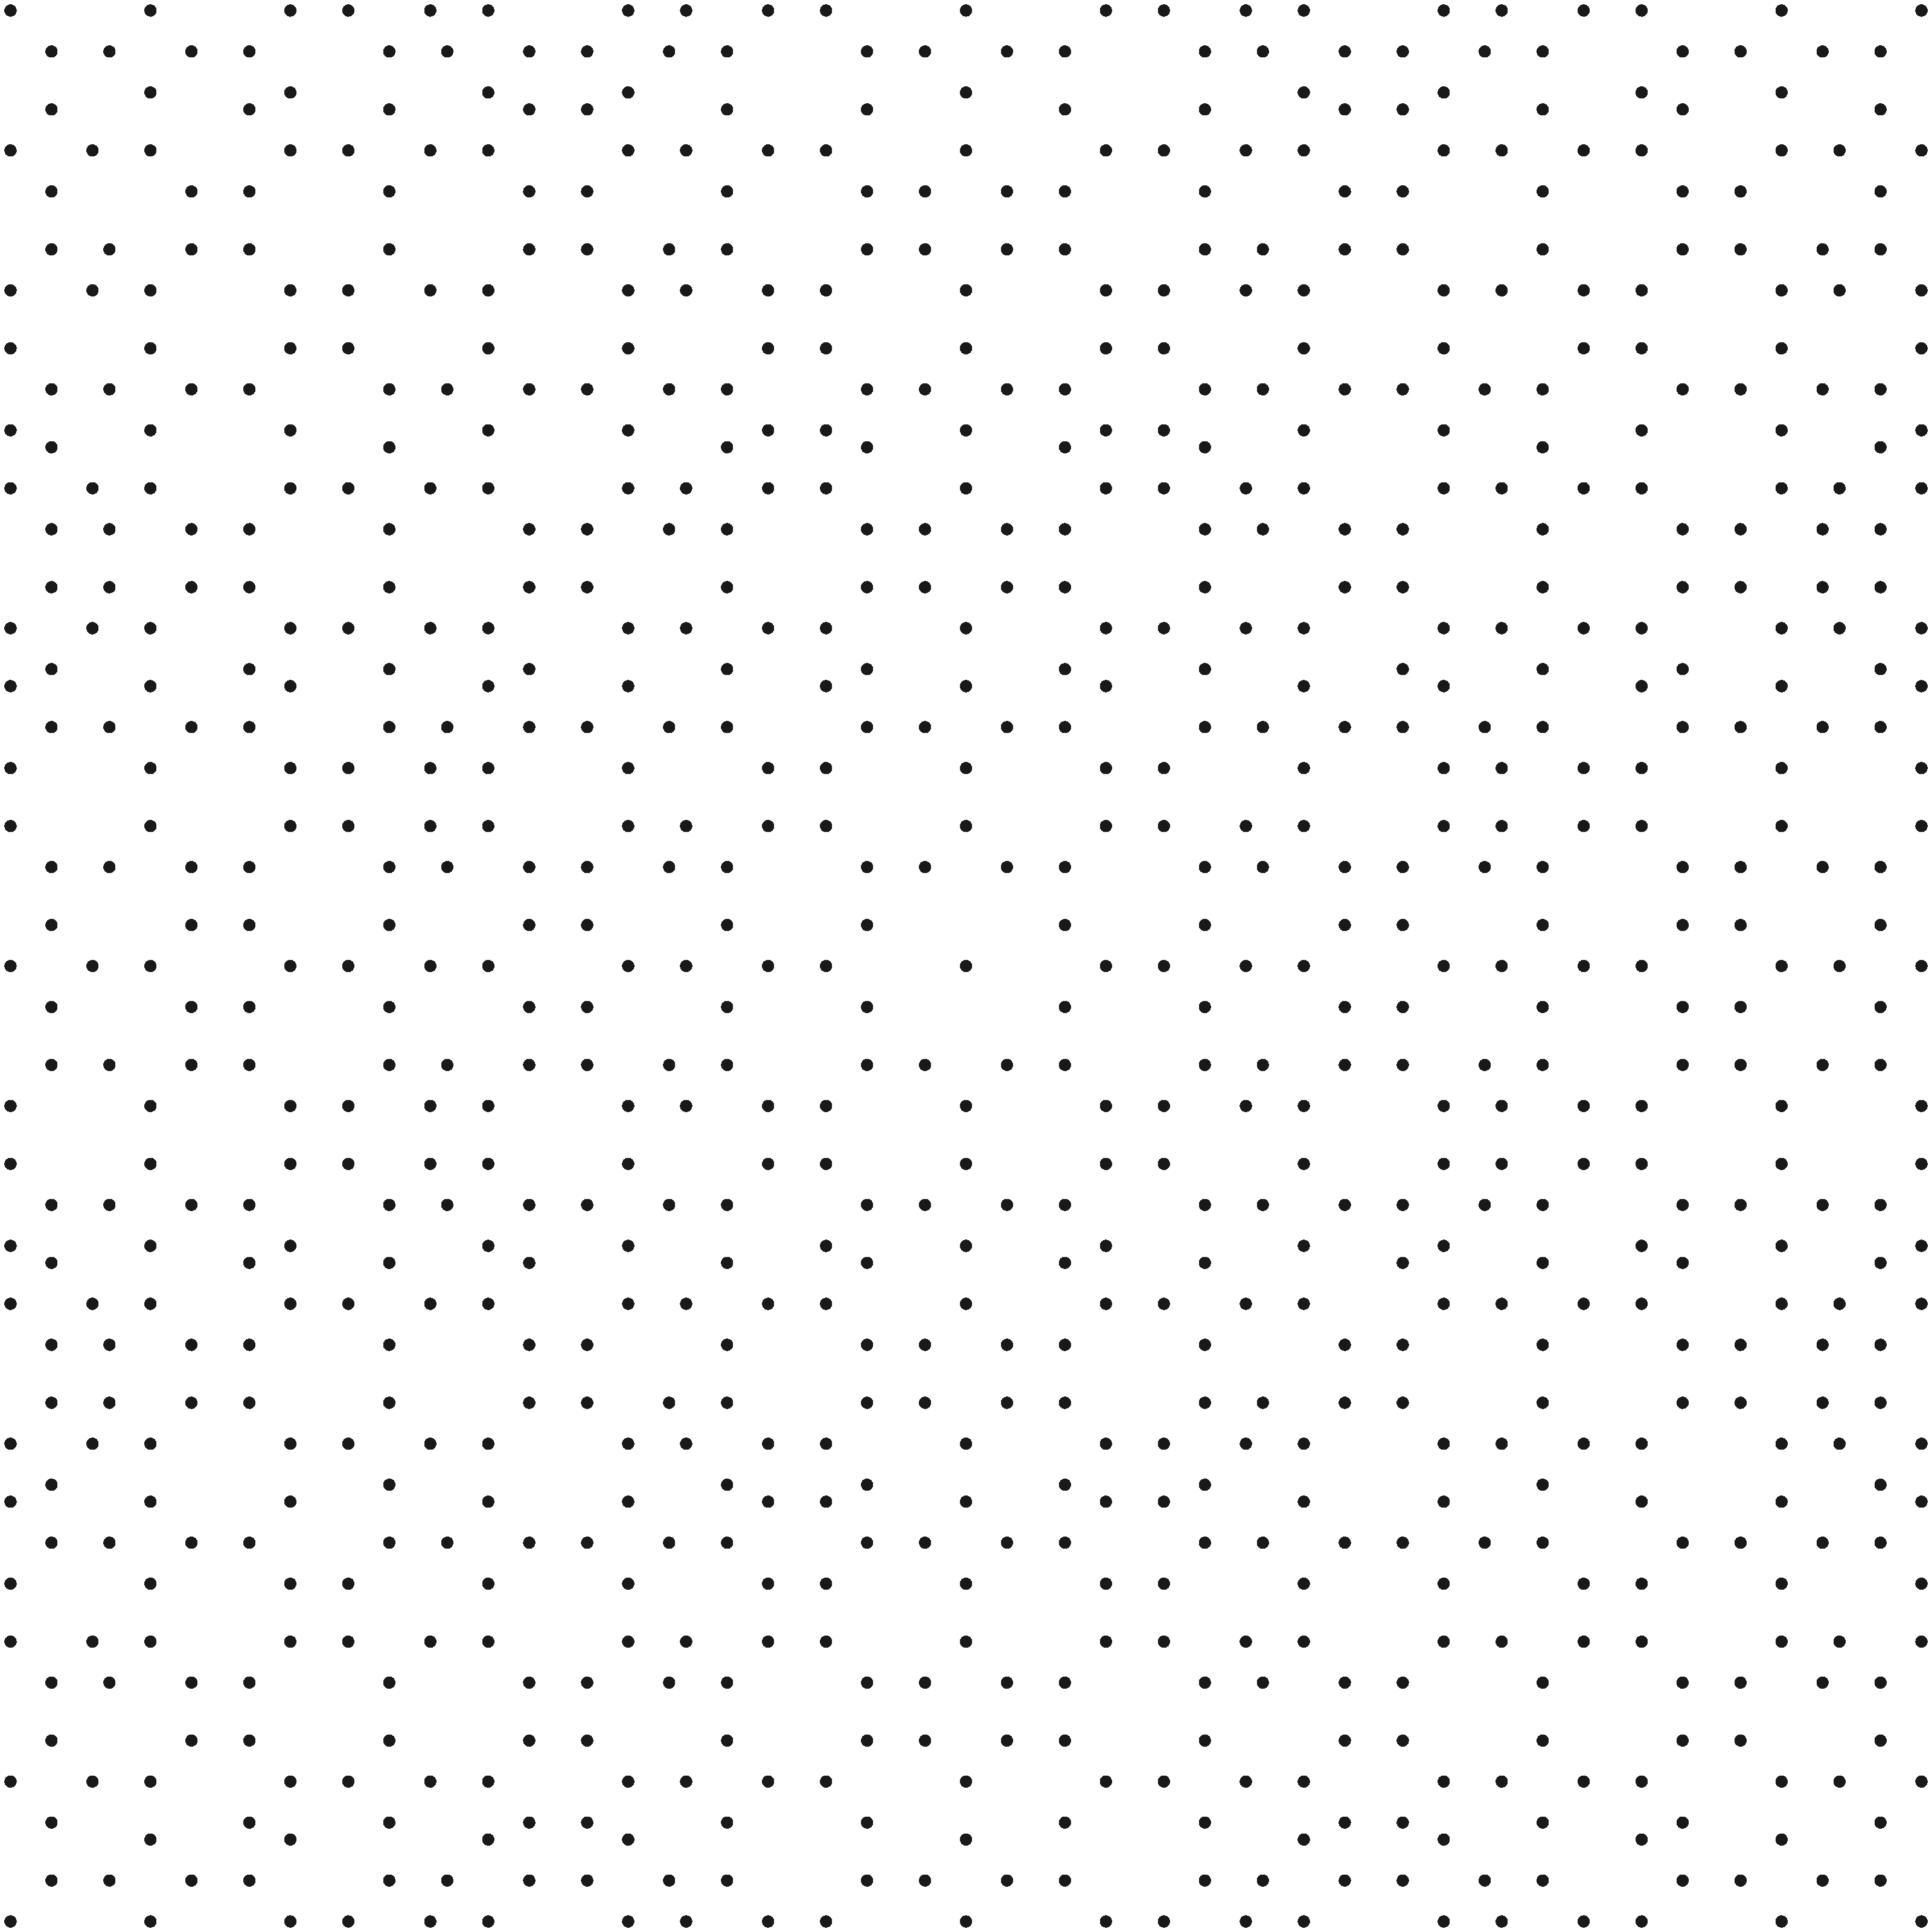
\includegraphics[width=0.9\textwidth]{img/firstExample}
\caption{Example of a two dimensional quasicrystal.}
\label{fig_quasicrystalFirstExample}
\end{figure}

To validate our quasicrystal model we of course have to show that it follows the attributes from Section \ref{sec_quasicrystalEaseIn}. However first we list few properties of our model which will help us show the validity of our model. 

\begin{itemize}
\item Inclusion property: $$\Omega_1\subset\Omega_2 \quad\Rightarrow\quad \quasi{\Omega_1}\subset\quasi{\Omega_2}$$
\item Union property: $$\quasi{\Omega_1\cup\Omega_2} \,=\, \quasi{\Omega_1}\cup\quasi{\Omega_2}$$
\item Translation property: $$\quasi{\Omega+x^\ast} \,=\, \quasi{\Omega}+x\qquad \text{for}\; x\in M$$
\item Scaling property: $$\quasi{\beta\Omega} \,=\, \beta'\quasi{\Omega}$$
\end{itemize}

And now to validate our model. 

\begin{enumerate}
\item uniform discreteness: $$\exists\,r_1>0,\; \forall z_1,z_2\in\Lambda, z_1\neq z_2:\; |z_1-z_2|>r_1$$
\item relative density: $$\exists\,r_2>0,\; \forall z\in\CC:\; B(z,r_2)\cap\Lambda \neq \emptyset$$
The result of the cut-and-project scheme is a Delone set \cite{lagarias} if the window $\Omega$ is bounded with nonempty interior, which is how we defined it. 
\item finite local complexity: $$\big|\{V(x)-x\,|\, x\in \Lambda\}\big|<\infty$$
It has been shown \cite{lagarias} that our model has even this property, however since our work explores the list of Voronoi tiles we essentially prove this in the process. 
\item rotational symmetry: $$\exists\,\zeta = e^{2\pi \i/n}:\; \zeta\Lambda^\CC = \Lambda^\CC$$
Rotational symmetry appears in quasicrystal if the window $\Omega$ has the same rotational symmetry.
\item dilation: $$\exists\,b\in\RR\setminus\{-1,1\}:\; b\Lambda\subset \Lambda$$
Using the scaling property and the inclusion property:
$$\beta\quasi{\Omega} = \quasi{\beta'\Omega} \subset \quasi{\Omega}$$
\end{enumerate}

Having quasicrystal defined and  our model validated, we shall present our plan for the analysis. 

\section{General quasicrystal analysis}
In this section we will outline a general method of analysis of any quasicrystal. Later we will use this method to analyze two dimensional quasicrystals. 

Analysis should reveal the structure of the points of the quasicrystal, for us that means acquiring the list of Voronoi tiles for each quasicrystal. 

To acquire such list we follow these steps: 
\begin{enumerate}
\item \textbf{Acquire arbitrary finite section of the quasicrystal}

In other words this means creating an algorithm that for a finite section $P\subset\RR^d$ returns $P\cap\quasi{\Omega}$. 
\item \textbf{Estimate the covering radius $R_C$ of the quasicrystal}

We are specifically interested in the upper bound $\hat{R}_C$ of the covering radius. This is necessary since in a Delone set Voronoi tile's domain's points can be no further from the center then double of the covering radius. 
\item \textbf{Generate a superset of all finite sections spanning $B(2\hat{R}_C)$}

Each of these finite sections represents one Voronoi tile that appears in the quasicrystal's voronoi diagram. 
\item \textbf{Filter the superset to the final list of Voronoi tiles}

Due to technical constrains previous step may have created more tiles than there actually are in the list of Voronoi tiles and so it needs to be filtered. 
\end{enumerate}

There is also a sort of a fifth step of the analysis that is no longer fixed on a single window of certain size, but explores the changes in the quasicrystal with changing window size. 
\begin{enumerate}
\setcounter{enumi}{4}
\item \textbf{Establish the period of each Voronoi tile}

A Voronoi tile generally appears in quasicrystals for whole interval of window sizes. Goal of this step is to establish the endpoints of such interval. 
\end{enumerate}

These steps are general enough to analyze any quasicrystal linked to any Pisot-cyclotomic number and in any dimension. Unfortunately, they are also too general and we will need to specify them for each specific quasicrystal. 

We close this chapter and our general overview of quasicrystals with discussion of window shapes. It is obviously impossible to analyze a quasicrystal for arbitrary bounded $\Omega\subset N$ with nonempty interior. That is however not necessary. Not every two windows generate different quasicrystals, especially since we do not consider translated and/or $\beta$~inflated quasicrystals to be different. 

\subsection{Analyzed window shapes}
We will use the properties of quasicrystals to gradually limit the set of analyzed windows. We start with all of the windows: 
$$\big\{\Omega\,|\, \Omega\subset N ,\;\text{bounded with nonempty interior}\big\}$$

To maintain our sanity we first limit our scope to convex bounded windows with nonempty interior. 
$$\big\{\Omega\,|\, \Omega\subset N ,\;\text{convex bounded with nonempty interior}\big\}$$

Further thanks to the translation property we can limit our scope to convex bounded windows with nonempty interior centered around the origin: 
$$\big\{\Omega-C_\Omega\,|\, \Omega\subset N ,\;\text{convex bounded with nonempty interior}\big\}$$
where $C_\Omega$ is the centroid or geometric center of the window $\Omega$. 

Lastly thanks to the scaling property we can limit our scope to convex bounded windows with nonempty interior centered around the origin of diameter in $(1,\beta]$:
$$\big\{\Omega-C_\Omega\\,|\, \Omega\subset N ,\; d(\Omega)\in (1,\beta] ,\;\text{convex bounded with nonempty interior}\big\}$$
where $d(\Omega)$ is the set diameter $d(\Omega) = \sup\{d(x,y)\,|\,x,y\in\Omega\}$, where $d(x,y)$ is the distance between $x$ and $y$. 

\begin{remark}
We could of course also pick any other $\beta$ multiple of $(1,\beta]$. 
\end{remark}

Of course even after all this limiting, the set of windows is still infinite. Therefore we will further limit our scope to three basic window shapes: rhombus, regular $n$-gon and a circle. The rhombus is not really a valid window since it is not sufficiently rotationally symmetrical, it is however fundamental to our method, more on this later. The regular $n$-gon represents the simplest window with sufficient rotational symmetry and the circle is interesting for its circular symmetry. 

To summarize we will analyze quasicrystals for windows in shape of rhombus, regular $n$-gon and a circle centered around the origin of diameter in $(1,\beta]$. Technically there is an infinite amount of these windows as well however as we will see later it is already manageable. 

Finally we need to discuss the boundaries of the windows. Generally we will assume closed windows i.e.\ we will include the boundary. The exception is the rhombus for reasons we will also explain later. 

Now we have quasicrystal defined, model explored and windows limited. In the next chapter we will finally start the analysis. 
\end{document}
